%
%  original proposed schedule, for reference
%
\section{Proposal Plan}
\label{sec:prop-plan}

For reference, the ``new'' HOPS project was proposed with
a 4-year timeline with funds adequate to support one FTE.
The proposal, notional schedule is shown in
Fig.~\ref{fig:prop-quarterly}.
\begin{figure}[!h]
\center{\fbox{%
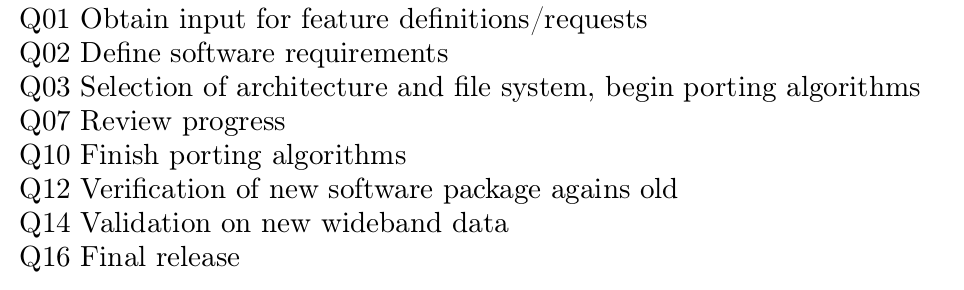
\includegraphics[width=0.70\textwidth]{nuHOPStimeline}}}
\caption[Proposed Quarterly Plan]{%
This snippet from the proposal shows the original quarterly
plan of develop for the ``new'' HOPS project.  Notionally the
project kicked-off Oct 1, 2019, so Q1 is Oct--Jan of that
year.  Notionally, then the final quarter, Q16 is July--Sep
of 2023.  }
\label{fig:prop-quarterly}
\end{figure}
As everyone is aware, COVID-19 changed many things as discussed
in the main body of the text.  After the proposal was accepted,
the work was waterfalled into a Gantt format
(see Fig.~\ref{fig:ganttcrap}) which is useful only
to establish that the tasks proposed are plausible for the time
allowed.  As discussed in the body of the text, we shall be using
an agile development methodology which does not waterfall nicely.
\begin{figure}[!h]
\center{\fbox{%
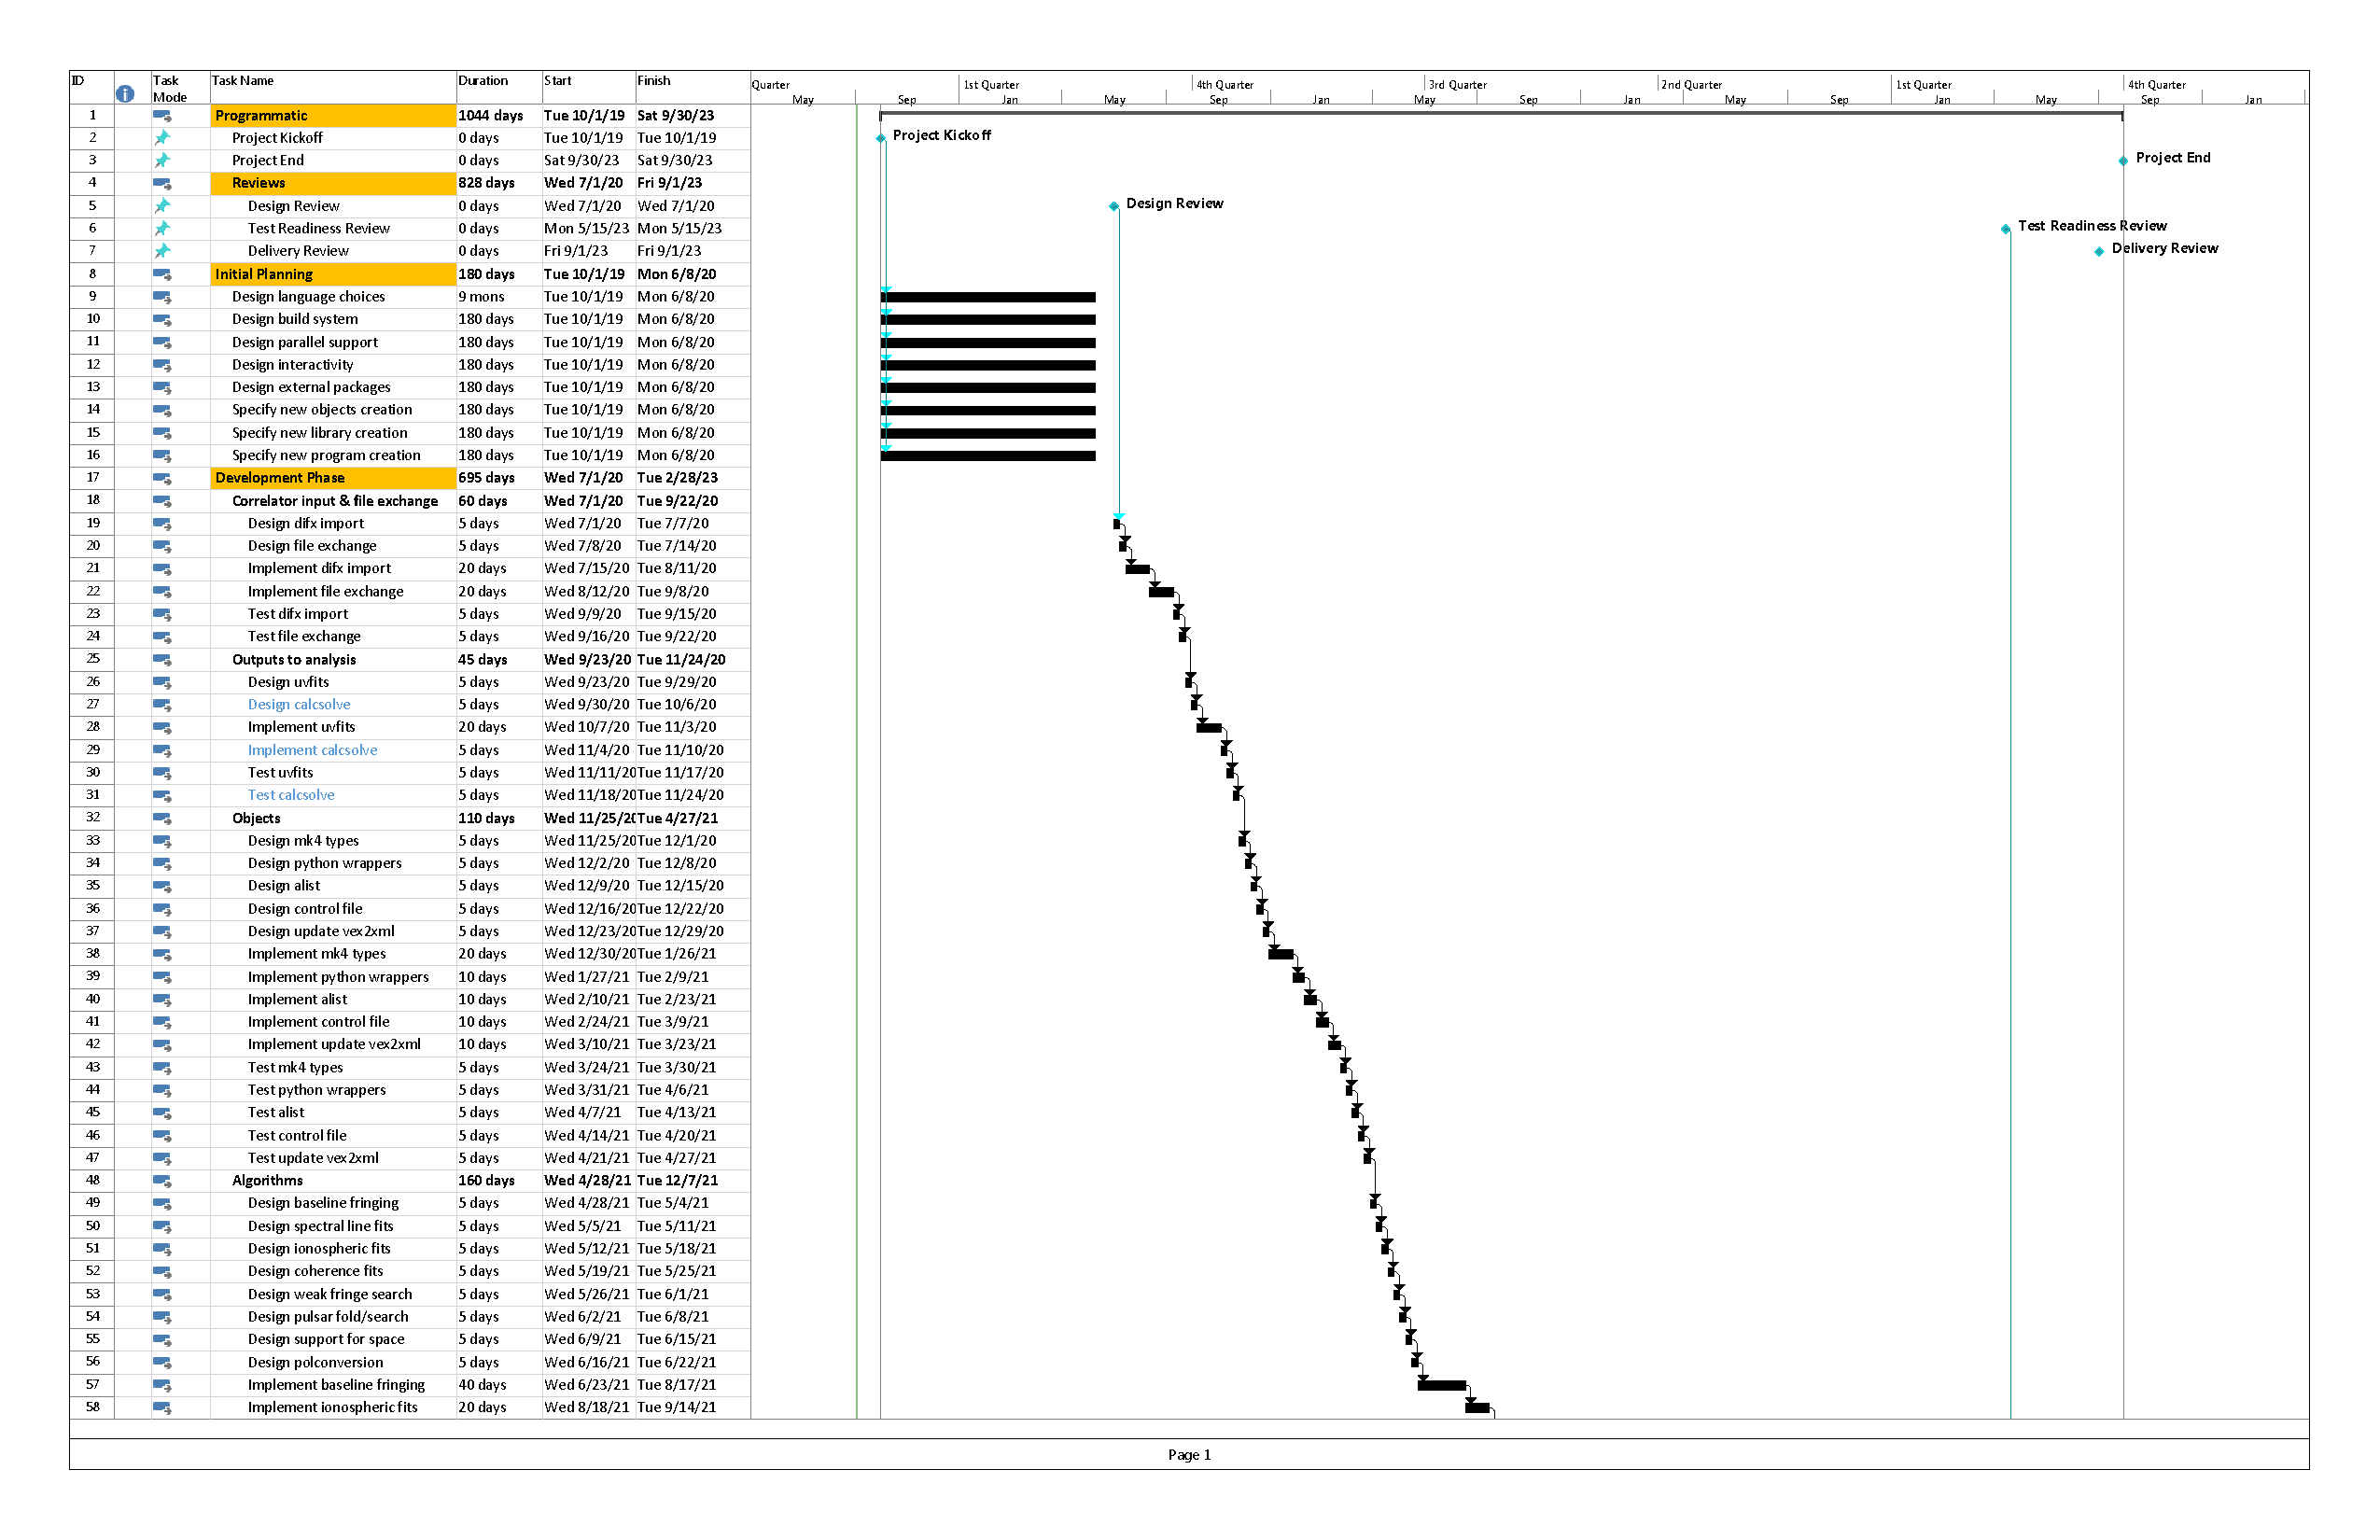
\includegraphics[width=0.40\textwidth]{MSRI-task-origv3-1}
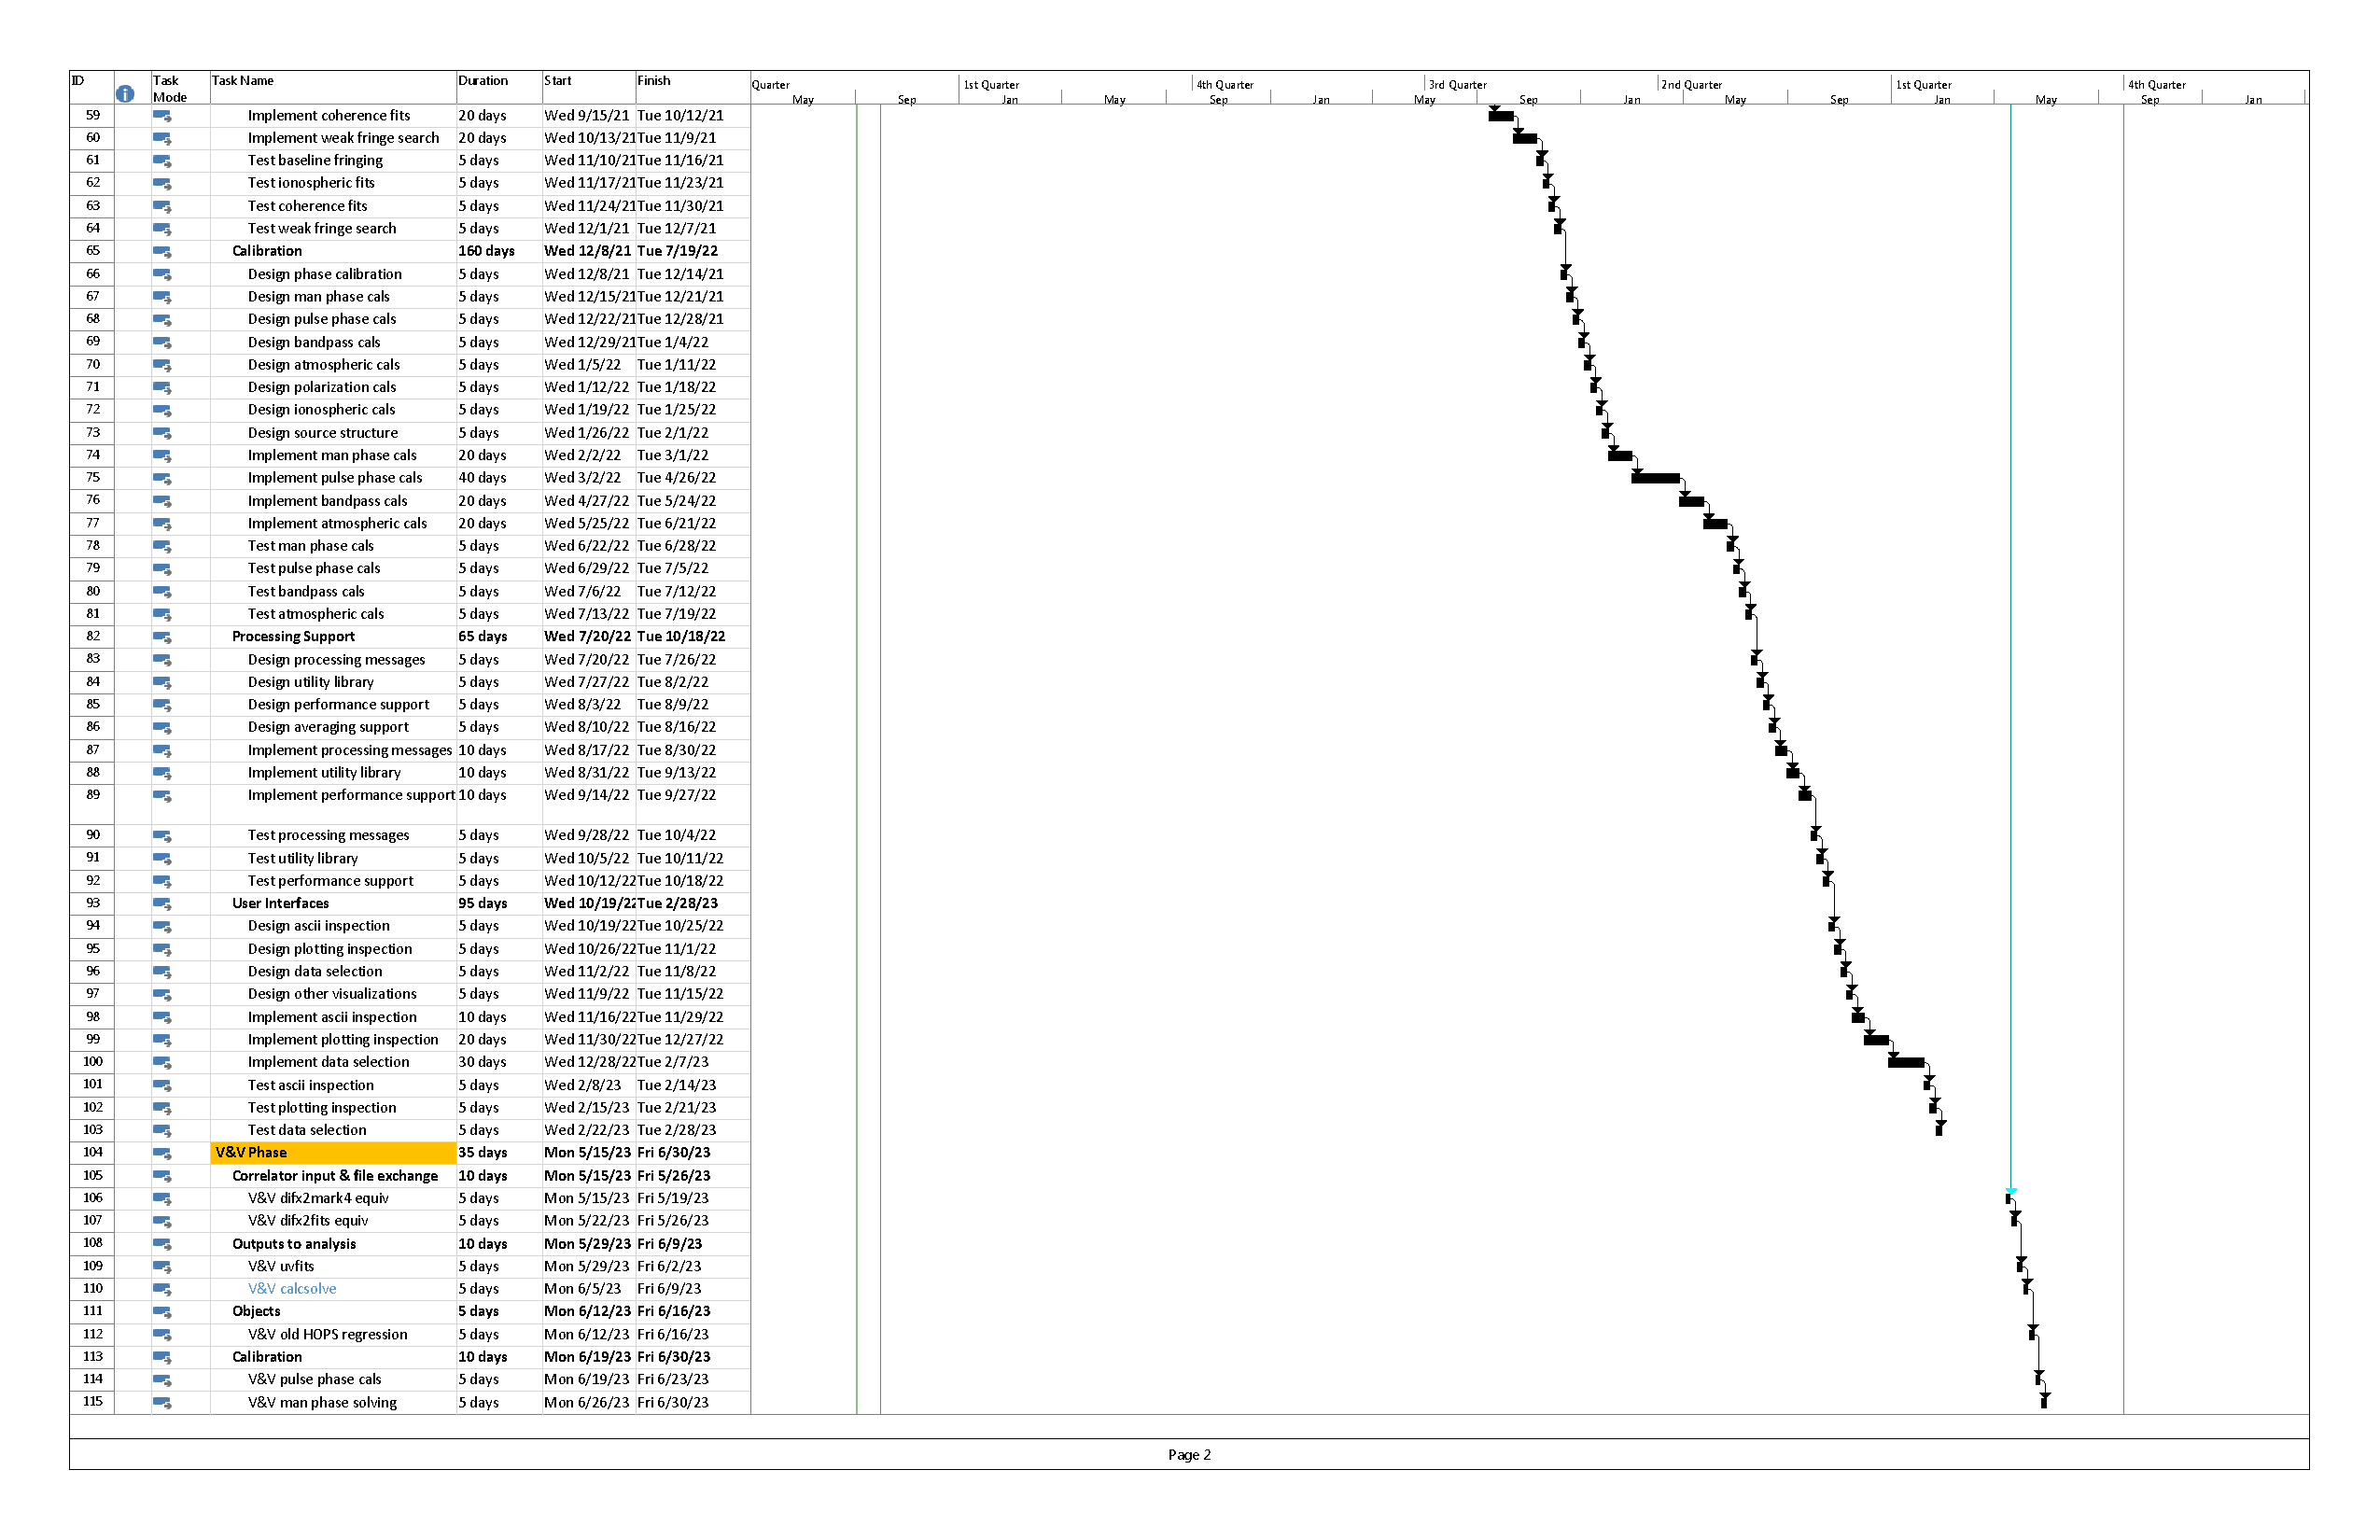
\includegraphics[width=0.40\textwidth]{MSRI-task-origv3-2} }}
\caption[Initial Gantt Timeline]{%
At the outset, a waterfalled Gantt-formulation of the work was
made to show that the 4-year timeline and estimated work effort
was consistent. The left panel corresponds to Q01--Q08, and the
right panel corresponds to Q09--Q16.}
\label{fig:ganttcrap}
\end{figure}

%
% eof
%
